\section{Farbgestaltung von Webseiten}
\label{sec:farbgestaltung}
Die Ziele der farblichen Gestaltung im Rahmen dieser Arbeit sind Lesbarkeit und Benutzerführung. Konkrete Kriterien für die Textlesbarkeit werden in \autoref{sec:lesbarkeit} vorgestellt. In  \autoref{sec:usability} wird der Begriff Benutzerführung erläutert und damit im Zusammenhang stehende Gestaltungsprinzipien im Webdesign herausgearbeitet. Davon ausgehend wird in \autoref{sec:architecture} ein konkreter Vorschlag für eine Systemarchitektur zur automatisierten Farbgestaltung von Webseiten erarbeitet.

\subsection{Lesbarkeit}
\label{sec:lesbarkeit}

\begin{figure}[]
	\centering
	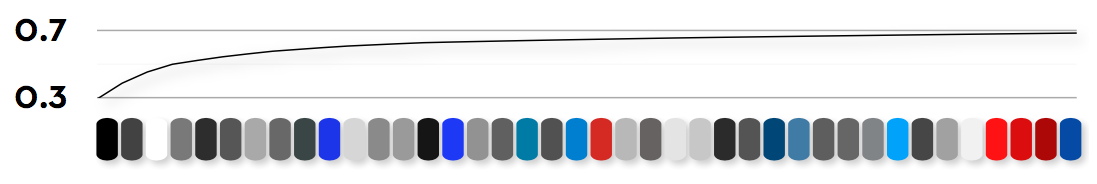
\includegraphics[width=0.7\textwidth]{img/webzeitgeist_textcolors.png}
	\caption{Die 40 populärsten Textfarben in Webseiten machen $70\%$ aller verwendeten Textfarben aus. (Quelle: \citep{webzeitgeist})}
	\label{fig:webzeitgeist_textcolors}
\end{figure}

\autoref{fig:webzeitgeist_textcolors} zeigt, dass gemäß einer Auswertung von über 100.000 Webseiten Text in HTML-Dokumenten fast ausschließlich in Graustufen dargestellt wird \citep{webzeitgeist}. Die populärsten Farben sind Schwarz, Dunkelgrau und Weiß. \citet{webdesign} begründet dies damit, dass Text schlechter lesbar wird, je bunter er ist. Der Style Guide von Googles Material Design \citep{google} hebt hervor, dass Aufgrund des Simultankontrasts die Verwendung von Grau als Textfarbe bei Hintergrund mit hoher Buntheit zu unerwünschten Effekten führt, wie Abbildung \ref{fig:text_color} veranschaulicht. Stattdessen wird in Abhängigkeit von der Helligkeit des Hintergrunds die Verwendung von Schwarz bzw. Weiß mit einem Alpha-Wert (Transparenz) empfohlen. Konkret werden folgende Werte genannt:
\begin{enumerate}
	\item Dunkle Schrift: $\text{rgba}(0, 0, 0, 0.87)$
	\item Helle Schrift: $\text{rgba}(255, 255, 255, 1.0)$
\end{enumerate}

\begin{figure}[h]
	\centering
	
\includegraphics[width=0.95\textwidth]{img/text_color.png}
	\caption{Empfohlene Textfarbe bei buntem Hintergrund. (a) Textfarbe $\text{rgb}(114,114,114)$. Der Text ist aufgrund des Simultankontrasts unangenehmer zu lesen. (b) Textfarbe $\text{rgba}(0, 0, 0, 0.54)$, d.h. Schwarz mit einem Alphawert  von $54\%$. Die Textfarbe ergibt sich zu einer Verschwärzlichung der Hintergrundfarbe und vermeidet so den Simultankontrast. (Quelle: \citep{google})}
	\label{fig:text_color}
\end{figure}

Es ist zu entscheiden, wann die dunkle und wann die helle Textfarbe verwendet wird. Hierfür geben die Web Content Accessibility Guidelines (WCAG) des W3C konkrete Grenzwerte für Kontrastverhältnisse in Abhängigkeit von der Text-, der Hintergrundfarbe sowie der Textgröße an. Die Formel zur Berechnung des Kontrastverhältnisses $L_c$ lautet \citep{wcag-contrast}:

\begin{equation}
	\begin{split}
		L_c(e.c_\text{text}, e.c_\text{background}) = \frac{L(e.c_\text{text}) + 0.05}{L(e.c_\text{background}) + 0.05} \;,\\
		L(e.c_\text{text}) \geq L(e.c_\text{background})
	\end{split}
\end{equation}

mit $L_c \in [1, ... , 22]$, wobei $L_c(rgb(255, 255, 255), rgb(0, 0, 0)) = 22$ und $e.c_\text{text} = e.c_\text{background} \implies L_c(e.c_\text{text}, e.c_\text{background}) = 1$ gilt. Die Berechnungsvorschrift der normalisierten relativen Luminanz $L()$ einer Farbe ist \citep{wcag-rel-luminance} zu entnehmen.

Es gibt zwei verschiedene Grenzwertklassen \citep{wcag}. Die Grenzwertklasse \emph{AA} beschreibt die Minimalanforderung an lesbaren Text:
\begin{equation}
  	AA: L_c(e.c_\text{text}, e.c_\text{background}) \geq
	\begin{cases}
	3.0, \; \text{size}(e) \geq 18\text{pt} \lor \text{size}(e) \geq 14\text{pt} \land \text{weight}(e) = \text{bold}\\
		4.5,  \;  \text{sonst}
	\end{cases}
\end{equation}

Die Klasse \emph{AAA} beschreibt bessere Lesbarkeit durch die Verwendung höherer Grenzwerte:

\begin{equation}
  	AAA: L_c(c_1, c_2) \geq
	\begin{cases}
		4.5, \; \text{size}(e) \geq 18\text{pt} \lor \text{size}(e) \geq 14\text{pt} \land \text{weight}(e) = \text{bold}\\
		7.0,  \;  \text{sonst}
	\end{cases}
\end{equation}

\subsection{Benutzerführung}
\label{sec:usability}
Ein adäquater Farbeinsatz ermöglicht die Steuerung von Aufmerksamkeit und unterstützt die Bildung von Zusammenhängen \citep{webdesign}.  Dieses Konzept wird auch als visuelle Hierarchy bezeichnet \citep{visual-hierarchy}, bei welchem die Oberflächenelemente bei der Wahrnehmung strukturiert und priorisiert werden.
\citet{webdesign} unterteilt folgende Möglichkeiten zur Benutzerführung durch Farbeinsatz:

\begin{itemize}
	\item \textbf{Themengruppen:} Bedeutet die farbliche Kodierung inhaltlich definierter Bereiche. Hierbei handelt es sich um eine vom Gestalter erfundene, subjektive Farbsystemlogik. Sie stellt kein System, sondern eine Gestaltungsstuktur dar, die dem Anwender zu lernen aufgezwungen wird. Dies resultiert automatisch in Buntheit, welche Aufmerksamkeit erregt und somit kontraproduktiv für die Bildung einer visuellen Hierarchie ist. Aus diesen Gründen ist von dieser Variante abzuraten. Abbildung \ref{fig:theme_coding} verdeutlicht dies am Beispiel eines Online-Magazins.
	\item \textbf{Funktionsbereiche:} Bedeutet die farbliche Abgrenzung von Bereichen mit einheitlicher Funktion. Dies beinhaltet beispielsweise die farbliche Differenzierung von Navigations-, Inhalts- und Servicebereichen. Diese Variante ist zu empfehlen, wenn nicht mehr als drei Farben verwendet werden und die betreffenden Bereiche gleichzeitig und somit im Bezug zueinander sichtbar sind. Abbildung \ref{fig:functional_areas} verdeutlicht dies am Beispiel der farblichen Abgrenzung verschiedener Navigationsbereiche.
	\item \textbf{Funktionen und Zustände:} Bedeutet die farbliche Kodierung verschiedener Elemente mit einheitlicher Funktion. Beispielsweise sind alle anklickbaren Elemente (z.B. Links und Buttons) einer Seite durch eine einheitliche Farbe signalisierbar. Abbildung \ref{fig:functions} zeigt hierfür ein Beispiel. Bestimme Wirkungen können zusätzlich farblich hervorgehoben werden, wie z.B. die rote Färbung von Buttons zum Löschen oder Abbrechen einer Aktion. Wurde eine Farbe einmal mit einer Funktion belegt, soll sie einheitlich verwendet werden. Beispielsweise würde ein nicht-anklickbares, blaues Element in der Oberfläche aus Abbildung \ref{fig:functions} den Nutzer verwirren.
\end{itemize}

\begin{figure}[]
	\centering
	
\includegraphics[width=0.48\textwidth]{img/theme_coding.png}
	\caption{Farbkodierung von Themengruppen am Beispiel von \url{www.smashingmagazine.com/}. Es ist unklar, weshalb die gewählten Farben mit den jeweiligen Bereichen assoziiert werden.}
	\label{fig:theme_coding}
\end{figure}

\begin{figure}[]
	\centering
	
\includegraphics[width=0.48\textwidth]{img/functional_areas.png}
	\caption{Farbkodierung von Funktionsbereichen am Beispiel von \url{www.leipzig-studieren.de}. Navigationsbereiche (orange) werden zueinander in Bezug gebracht und vom Inhalt (weiß) abgegrenzt.}
	\label{fig:functional_areas}
\end{figure}

\begin{figure}[]
	\centering
	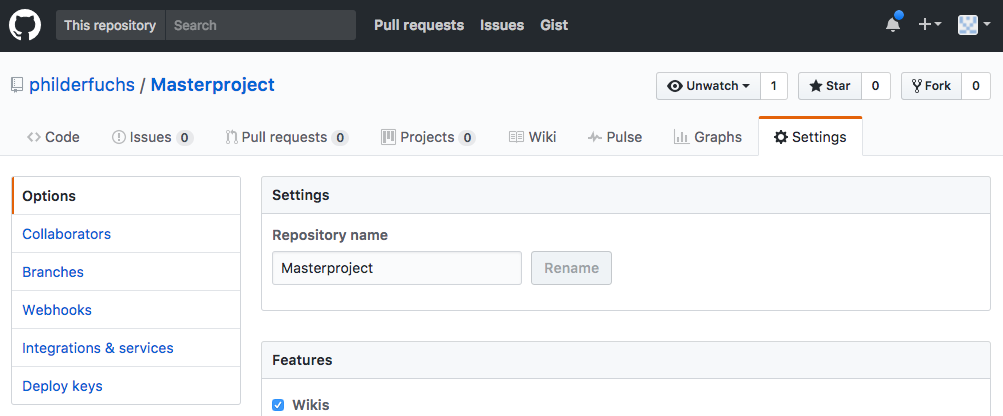
\includegraphics[width=0.48\textwidth]{img/functions.png}
	\caption{Farbkodierung von Funktionen am Beispiel von \url{www.github.com}. Nur anklickbare Elemente sind blau, aktive Elemente werden zusätzlich braun markiert.}
	\label{fig:functions}
\end{figure}

\subsubsection{Farbfunktionen}
Aus \autoref{sec:usability} geht hervor, dass Elemente entsprechend ihrer Funktion gefärbt werden, nicht aus rein dekorativen Gründen oder zur thematischen Strukturierung. Aus diesen Gründen wird zwischen die Abbildung $CGs \to P$ eine Abstraktionsschicht mit der Bezeichnung \textbf{Farbfunktionen} $F$ geschoben, welche beschreibt, welche Funktion eine Color Group in einer Oberfläche erfüllt. In Anlehnung an \citep{google,  smashing} wird exemplarisch $F = \{\text{Primär}, \text{Sekundär}, \text{Interaktion}, \text{Akzent}, \text{Text Hell}, \text{Text Dunkel}, \text{Hintergrund}\}$ definiert. Die einzelnen Farbunktionen lauten wie folgt:
\begin{itemize}
	\item \textbf{Primärfarbe:} Wird in Relation zu den anderen Farben am häufigsten eingesetzt und bildet so die farbliche Grundstimmung der Oberfläche \citep{awwwards}.
	\item \textbf{Sekundärfarbe:} Unterstützt die Farbstimmung der Primärfarbe und orientiert sich dementsprechend an deren Farbton. Durch die Wahl einer unbunteren Farbe tritt sie in der visuellen Hierarchie stärker in den Hintergrund \citep{visual-hierarchy}, eignet sich besser als Hintergrund für Fließtext und unterstützt durch den Qualitätskontrast die Wirkung der Primärfarbe \citep{webdesign}.
	\item \textbf{Interaktionsfarbe:} Signalisiert Elemente, mit denen eine Interaktion möglich ist, z.B. klicken. Dies trifft nicht zwangsläufig auf Elemente zu, bei denen der Nutzer eine Interaktionsmöglichkeit aufgrund ihrer Funktionsgruppe bereits erwartet, wie z.B. in der Seitennavigation.
	\item \textbf{Akzent:} Signalisiert Elemente mit hoher Priorität in der visuellen Hierarchie. Dies ist erreichbar durch einen relativ seltenen (Quantitätskontrast, \citep{webdesign}) Einsatz einer bunten \citep{visual-hierarchy} Farbe.
	\item \textbf{Text Hell/Dunkel:} Farbe für Fließtext. Entsprechend \autoref{sec:lesbarkeit} wird hierfür in Abhängigkeit Hintergrund Weiß (Hell) bzw. Schwarz (Dunkel) mit Alpha-Kanal festgelegt.
	\item \textbf{Hintergrund:} Standardfarbe von Blöcken, die keiner der obigen Farbfunktionen entsprechen. Dies betrifft vorwiegend Blöcke mit Fließtext, so dass Textlesbarkeit zu beachten ist. Dementsprechend sind Graustufen zu bevorzugen \citep{webx0}, wobei entsprechend \autoref{sec:lesbarkeit} ein ausreichender Luminanzkontrast zu gewährleisten ist. Darum wird die Hintergrundfarbe analog zur Textfarbe auf Weiß bzw. Schwarz festgelegt.
\end{itemize}

Die hier verwendeten Farbfunktionen sind exemplarisch. Abhängig von den individuellen Ansprüchen einer Webseite ist die Definition weiterer Farbfunktionen denkbar. Bei mobilen Anwendungen ist beispielsweise eine farbliche Differenzierung verschiedener Interaktionsformen sinnvoll (z.B. drücken und wischen).
Die Abbildung zwischen Color Groups und Farbfunktionen wird als die Funktion $S$ definiert und im folgenden als \textbf{Farbschema} definiert. Es gilt: 
\begin{equation}
  S: F \to P
\end{equation}

Diese Definition eines Farbschemas unterscheidet sich von der Verwendung des Begriffs in der Literatur \citep{webdesign}. In dieser ist ein Farbschema eine Charakterisierung einer Farbpalette. Es beschreibt, \emph{wie viele} unterschiedliche Farbtöne eine Farbpalette enthält und in welcher \emph{geometrischen Beziehung} diese zueinander stehender.  Beispielsweise bezeichnet ein \emph{triadisches} Farbschema eine Farbpalette mit drei Farbtönen, die sich in einem Abstand von $120^{\circ}$ zueinander befinden. Genauer wird in  \emph{monochromatische}, \emph{komplementäre (duale)}, \emph{triadische} und \emph{tetraedische} Farbschemen unterschieden, welche Farbpaletten mit einem, zwei, drei oder vier verschiedenen Farbtönen repräsentieren. \citep{underestimated, smashing, google} empfehlen jedoch die Beschränkung auf höchstens 3 Farben im Webdesign, während Graustufen für die Darstellung von Text und Hintergründen dominieren. Dementsprechend werden die Begriffe \textbf{monochrom}, \textbf{dual} und \textbf{triadisch} für die Charakterisierung des Farbschemas als Farbabbildung in dieser Arbeit adaptiert.
    
\autoref{fig:colorschemes} zeigt hierfür Beispiele. Oben wird eine exemplarische \emph{Farbpalette} abgebildet. Die \emph{Farbfunktionen} entsprechen der in diesem Abschnitt definierte Menge $F$. Es ist zu erkennen, dass die Textfarben sowie die Hintergrundfarbe bereits pauschal definiert werden. Damit realisiert jedes Farbschema im Rahmen dieser Arbeit einen \textbf{Bunt-Unbunt-Kontrast}, was nach \citep{webx0} eine allgemeine Empfehlung für Webdesign darstellt. Die Abbildung zeigt weiterhin mögliche Abbildungen zwischen den Farbfunktionen und der Farbpalette unter \emph{Farbschemata}. Ein monochromes Farbschema beschränkt sich auf einen Farbton in verschiedenen Schattierungen. Dadurch wird ein \textbf{Qualitätskontrast} gebildet, welcher die Wirkung der Farbe mit dem höchsten Buntheitswert erhöht. Die inverse Variante des monochromen Schemas veranschaulicht eine Variante mit allgemein dunkler Farbstimmung. Das duale Farbschema besitzt zwei Farbtöne. Da Interaktions- und Akzentfarben weniger häufig auftauchen als die Elemente der Primär- und Sekundärfarben wird hierdurch ein \textbf{Quantitätskontrast} gebildet, der die seltenere Farbe zusätzlich betont und so zur Bildung einer visuellen Hierarchie beiträgt. Das exemplarische tertiäre Farbschema  bildet die Interaktions- und Akzentgruppen auf unterschiedliche Farben ab und differenziert diese so zusätzlich. 

\begin{figure}[h]
	\centering
	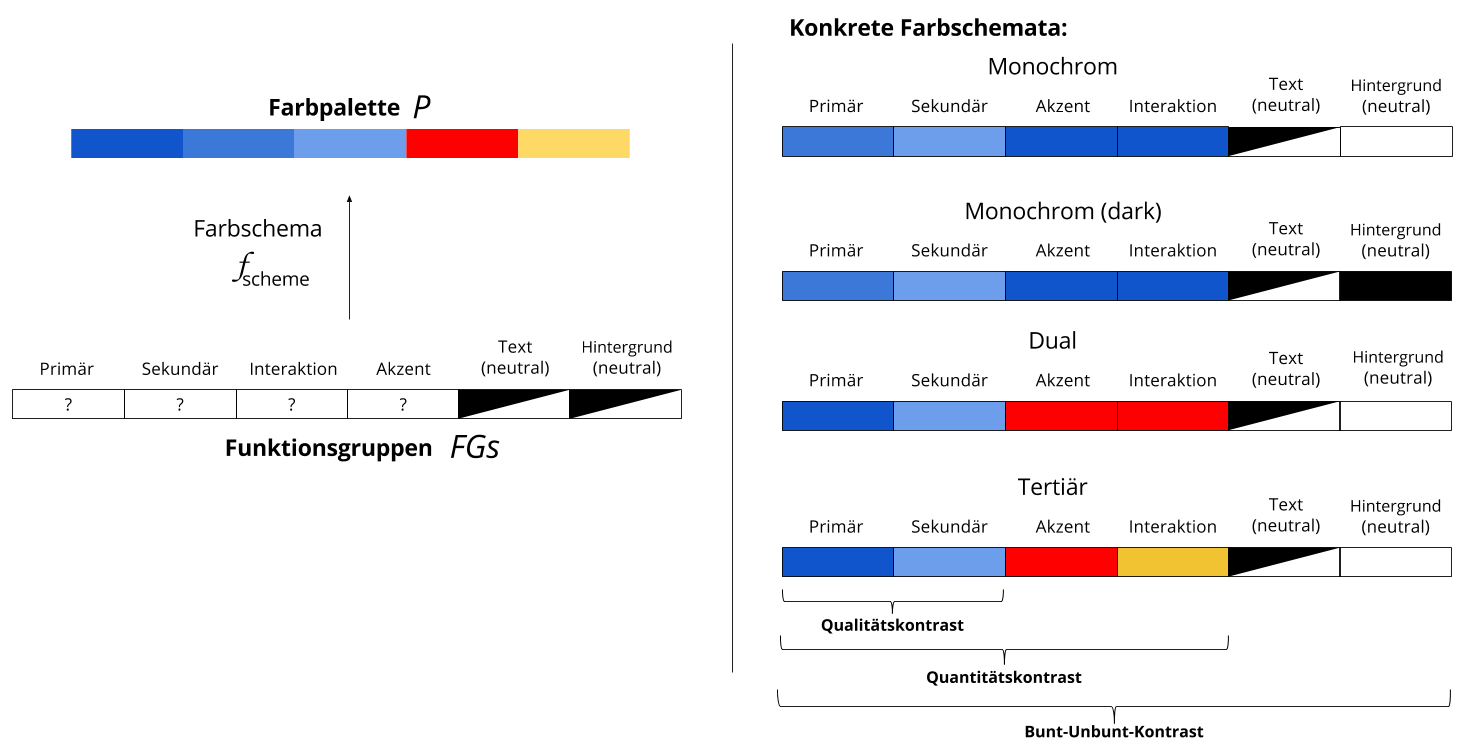
\includegraphics[width=0.48\textwidth]{img/colorschemes.png}
	\caption{Beispiele für monochrome, duale und tertiäre Farbschemata. Der Farbeindruck der Seite wird durch Quantitäts-, Qualitäts- und Bunt-Unbunt-Kontraste bestimmt.}
	\label{fig:colorschemes}
\end{figure}

\subsection*{Zusammenfassung}
Zur Unterstützung der Benutzerführung werden in Webseiten Funktionsbereiche und Elemente mit einheitlicher Funktion bzw. Funktionszustand farblich kodiert. Dementsprechend werden für eine Webseite eine Menge an Farbfunktionen $F$ definiert, wie z.B. die Interaktionsfarbe, welche klickbare Elemente signalisiert. Ein Farbschema $S: F \to P$ ist eine Abbildung der Farbfunktionen auf die Farben einer Palette $P$. Eine Abbildung soll höchstens drei verschiedene Farbtöne enthalten. Für Fließtext sowie dessen Hintergrund werden standardmäßig Graustufen festgelegt. Zur Benutzerführung realisieren Webseiten somit einen Bunt-Unbunt- sowie Quantitätskontrast, welcher das zentrale Gestaltungsmittel des Screendesigns darstellt \citep{webdesign, webx0}.